% Towards Adaptive Hand Prosthetics
% Castellini, Gruppioni, Davalli, Sandini
% submitted to IEEE Transaction on Robotics
% special issue on Rehabilitation Robotics
%
% September, 2008

\documentclass[journal]{IEEEtran}

\usepackage{times}
\usepackage{epsfig}
\usepackage{graphicx}
\usepackage{amsmath}
\usepackage[psamsfonts]{amssymb}
\usepackage{url}
\usepackage[pagebackref=true,breaklinks=true,letterpaper=true,colorlinks,bookmarks=false]{hyperref}

\def\RR{\mathbb{R}}
\def\NN{\mathbb{N}}
\def\xx{\mathbf{x}}
\def\yy{\mathbf{y}}
\def\ww{\mathbf{w}}

\begin{document}

\title{Towards Adaptive Hand Prosthetics}

\author{Claudio~Castellini, Emanuele~Gruppioni, Angelo~Davalli, Giulio~Sandini%
\thanks{C. Castellini \emph{(corresponding author)}
  is with the LIRA-Lab, University of Genova,
  viale F. Causa, 13, 16145 Genova, Italy.
  e-mail: claudio.castellini@unige.it.}%
\thanks{E. Gruppioni and A. Davalli
  are with the INAIL Centro Protesi,
  via Rabuina, 14, 40054 Vigorso di Budrio (Bologna), Italy.
  e-mail: \{e.gruppioni,a.davalli\}@inail.it.}%
\thanks{G. Sandini
  is with the RBCS Department, Italian Institute of Technology,
  via Morego, 30, 16163 Genova, Italy.
  e-mail: giulio.sandini@iit.it.}%
}

\maketitle

\begin{abstract}
  abstract
\cite{v-edbed-82}

\end{abstract}

\begin{IEEEkeywords}
  IEEEtran, journal, \LaTeX, paper, template.
\end{IEEEkeywords}

\IEEEpeerreviewmaketitle

\section{Introduction}
\label{sec:introduction}
Active prosthetic hands, driven by a motor to open and close the
``claw,'' have been around for many years.  Recently, however,
advances in mechatronics have improved such hands and currently
various prosthetic hands with 3 or more active degrees of freedom are
being put on the market.  Such hand developments are a result of
various robotic hands which are highly humanoid, light and gifted with
a number of degrees of freedom. Attempts in this sense include, e.g.,
the DLR prosthetic hand (\cite{Hua2006}---see Figure
\ref{fig:DLRHandII}), the CyberHand project \cite{cyberhand}, and the
i-LIMB hand by Touch Bionics \cite{ilimb}.

\begin{figure}
  \begin{tabular}{cc}
    \includegraphics[height=0.12\textheight]{figs/DLRHand-Ball-comp.jpg} &
    \includegraphics[height=0.12\textheight]{figs/DLR-Prothese.jpg}
  \end{tabular}
  \caption{(left) The DLR Hand II. (right) The DLR prosthetic hand.}
  \label{fig:DLRHandII}
\end{figure}

Still, a general sense of frustration impends, as far as
\emph{control} of the prosthesis is concerned. As a matter of fact,
given the current state of the art, it is basically impossible for the
patient to precisely command the prosthesis what to do; whereas,
operating a hand requires a fine control down to the level of the
single fingers. First of all, presented with a certain task such as
turning a door handle or grabbing a car key, the patient must be able
to enforce the correct grasping type; this involves the activation of
some joints only, and in particular positions. Secondly, the amount of
force involved in the grasp must be controlled, so that it is possible
to grab, e.g., both a hammer without letting it slip and an egg
without breaking it.

To this end, two types of interfaces between the patient and the
prosthesis have been developed or are being studied: \emph{invasive}
and \emph{non-invasive}. The former gather control signals directly
from the user's nervous system, either via brain implants or surgical
use of electrodes. Quite obviously, invasive interfaces are supposed
to deliver a high signal quality, since the signals can be gathered
exactly in the right spots; but they involve surgery and all related
sterility (and psychological) issues. On the other hand, non-invasive
interfaces are easier to handle, manufacture and implant, but require
a much better signal conditioning, since they usually work with
surface (skin) signals or vision and gaze tracking.

In the context of non-invasive interfaces for controlling mechanical
hands, a concrete possibility arises from \emph{forearm surface
electromyography} (EMG), a technique by which muscle
activation potentials are gathered by electrodes placed on the
patient's forearm skin; these potentials can be used to track which
muscles the patient is willing to activate, and with what force.
Surface EMG is therefore, in principle, a cheap and easy way of
detecting what the patient wants the prosthesis to do.

Still, the EMG signal suffers from a number of problems, among which
the unprecise placement of the electrodes, signal drifting and change
due to sweat formation and muscular fatigue and cross-talking among
deep and superficial muscles. It seems, though, that good results can
be obtained via \emph{machine learning} techniques, as shown in, e.g.,
\cite{smagt}. In machine learning, one tries to approximate an unknown
function given its values in a number of samples; the application to
the current problem is exactly that of building a map relating EMG
activation potentials and muscle force, and therefore hand finger
movements.

Such a system must be highly adaptive, accurate and fast---possibly,
able to run in real time, as the patient is wearing the prosthesis.
Another very desirable characteristic is that the system should learn
automatically as the patient moves, being able to understand when new
portions of the input space are being explored, i.e., what new
movements are required of the prosthesis. But so far machine learning
applied to surface EMG has only been able to classify hand postures.
For example, the surface EMG signal can be used to detect whether the
patient is attempting a cylindric grasp or a two-finger grip
\cite{ekvall}; but no indication about the amount of force involved in
the grasping act is detected.

In this paper we show a rather detailed analysis of what machine
learning can do when applied to such a problem. Over several days, we have
gathered forearm surface EMG data while an able-bodied human subject
was gripping in four distinct ways a force sensor; we have then
trained three different machine learning systems to guess, from the
EMG signal,
\begin{enumerate}

  \item what kind of grasp the subject was doing, e.g., thumb and
    index finger, thumb and middle finger, thumb and ring finger or
    thumb and all other fingers; and

  \item how much force the subject was exerting, in order to
    understand whether the grasp was, e.g., a power grasp or rather a
    precision grip. Surprisingly, as far as we know, nobody has ever
    attempted so far to solve this problem, although it is well-known
    that the EMG is related to the force a muscle is exerting.

\end{enumerate}

The three approaches we have experimented with are:
(a) a simple feed-forward neural network with one hidden layer,
(b) a Support Vector Machine with radial basis function kernel
\cite{BGV92}, and (c) Locally Weighted Projection Regression
\cite{lwpr}. Our analysis consists of a preliminary phase in which
several models have been built in a batch fashion, in order to
understand how to deal with the non-stationarity of EMG. The most
interesting challenge has been how to filter out unwanted data, at the
same time keeping a high overall accuracy, both in classification and
regression. Later on, based upon the results obtained in the
preliminary phase, we have developed a simple but effective procedure
for selecting a subset of the samples on-the-fly, called \emph{Online
Uniformisation} (OU).

OU is based upon the simple idea of keeping a minimum inter-sample
Euclidean distance, in order to uniformly sample the input space. The
selected samples are then used to periodically re-train the system,
and check that it has adapted to the new data. The training sets thus
obtained are remarkably small and thus usable on-line, and they offer
an excellent trade-off between size and accuracy. In particular, as a
certain parameter is increased, the size of the uniform training sets
decreases polynomially, while the error rate increases only
linearly; therefore one can obtain much smaller training sets (which
means faster or more adaptive machines) by accepting an error rate
which is only linearly worse.

This behaviour appears in both problems highlighted above (the former
involving classification, the latter regression), and for all the
approaches tested. Our numerical results indicate that, in such a
scenario, the type of grasp can be reconstructed with an average
accuracy of $89.67\% \pm 1.53\%$, and the applied force can be
predicted with an average percentage error of $7.89\% \pm 0.09\%$,
meaning $4.5$N over a range of about $57$N.

The paper is structured as follows: after a brief review of relevant
literature, we describe in detail the experiment and the methods used
to tackle it (Section \ref{sec:m&ms}); then we show and comment on the
experimental results, both the preliminary phase and the online
experiments (Section \ref{sec:exp}); lastly, discussion and
conclusions are presented.


\section{Materials and Methods}
\label{sec:m&ms}
\subsection{Patients}

Three hand amputees, patients of the INAIL Centro Protesi in Vigorso
di Budrio, Bologna, Italy, joined the experiment.

The first subject is male, aged 63, trans-radial one-third proximal,
amputated in 1963; he is a pioneer of myoelectric prostheses, having
started using them in the Sixties. The second subject is male, aged
56, trans-radial one-third distal, amputated in 1972; he also started
using myoelectric prostheses very early, actually in 1974. The third
subject is male again, aged 25, trans-carpal, amputated in 2007; he
was in the process of learning how to use a standard myoelectric
prosthesis at the time of writing.

A set of three patients is obviously not sufficient to gather
statistics about the applicability of our method, but we are lucky
enough that they present a rather wide variety of operations and
conditions. In particular, subject $1$ has about $9$cm left of his
forearm, subject $2$ has some $20$cm, and subject $3$, a trans-carpal
amputee, has the whole forearm plus some of the carpus (Figure
\ref{fig:stumps} shows the subjects' stumps). Moreover, subjects $1$
and $2$ were amputated a very long time ago, although they have been
using myodevices since then, whereas subject $3$ is freshly
operated. Lastly, subject $3$ is rather young as opposed to the other
subjects.

\begin{figure*}[!ht] \centering
  \begin{tabular}{ccc}
    \includegraphics[width=0.3\textwidth]{figs/stump_1} &
    \includegraphics[width=0.3\textwidth]{figs/stump_2} &
    \includegraphics[width=0.3\textwidth]{figs/stump_3} \\
    subject $1$ & subject $2$ & subject $3$ \\
  \end{tabular}
  \caption{the subjects' stumps. Subject $1$ has a trans-radial
    one-third proximal amputation, with a stump about $9$cm long;
    subject $2$ is trans-radial one-third distal, stump about $20$cm
    long; and subject $3$ is trans-carpal, retaining the full
    forearm.}
  \label{fig:stumps}
\end{figure*}

\subsection{Setup}

We placed on each subject's stump $5$ surface EMG electrodes without
searching for the best anatomical position, but rather in a standard
way for all, around the stump, near the elbow (for subject $1$ this
was actually the only possible choice!) and at uniform angles from one
another, in such a way to "wrap" the stump. See the ``Discussion and
Conclusions'' Section for more about this issue.

The electrodes we employed are standard commercial surface EMG
devices, namely OttoBock Myobock models \cite{ottobock}, two of the
13C7=50 type and three of the 13E125=50 type. Myobock electrodes enjoy
an excellent noise rejection ratio and pre-amplify the signal --- an
amplification gauge can be set for each electrode, and here it was set
at a mid-range value for all electrodes. Moreover, they perform a
run-time root-mean square evaluation of the signal; this results in an
exceptionally good output, which is already highly correlated with the
force exerted by the muscle(s) whose activity the electrode is
gathering.

Each subject was also given a FUTEK LMD500 Hand Gripper force sensor
\cite{futek} in order to detect the required force during the
experiment. Data were gathered via a standard digital acquisition
card, namely a National Instruments NI-DAQ 6122 USB card, connected to
the EMG electrodes and force sensor on one side, and to an entry-level
laptop on the other side. We employed National Instruments's
SignalExpress application to sample the (synchronised) data at a
sampling rate of $100$Hz.

\subsection{Experiment Design}

The patients were induced to imagine performing with their missing
hand $5$ different postures / grips: no action, pointing index, pinch
grip, tripodal grip, power grasp; subject $3$ was also asked to
stretch his hand --- a posture which most amputees deem very useful
for, e.g., slipping the hand in a pocket. The postures / grips were
performed with free force and speed by the subjects, while we would
record the EMG and force sensor activity.

Since the beginning we decided to employ a \emph{supervised learning}
strategy to build our models, as has been done in literature so
far. To this end, three ways of training the system
(\emph{modalities}) were designed and employed:

\begin{enumerate}

  \item \emph{teacher imitation.} A healthy subject (the teacher)
    would place his arm besides the patient's stump and ask him
    to imagine replicating the teacher's postures and grips. The
    subject was asked to imagine gripping with his maximum strength,
    while the teacher would grip the force sensor in order to mark the
    postures / grips.

  \item \emph{bilateral action.} The patient was asked to grip the
    force sensor with his healthy hand while imagining doing the same
    things with his missing hand.

  \item \emph{mirror-box.} Same as modality $2$, but a simple, plain
    mirror (in the case of subject $1$), or a \emph{mirror-box} (for
    subjects $2$ and $3$, see \cite{mirror-box}), was placed
    in-between the patient's arms, in order to increase the visual
    feedback.

\end{enumerate}

The idea behind the mirror-box modality is inspired by Ramachandran's
experiments on amputees of the mid-Nineties \cite{ramachandran}, where
it was noted that the illusion of seeing one's hand moving would
reinforce the visual feedback loop and ease the ghost limb pain in
monolateral hand amputees. We figured out that such a device could
actually reinforce the patient's ability to produce different
activation patterns.

Figure \ref{fig:modalities} shows various subjects performing the
required actions in the three modalities.

\begin{figure*}[!ht] \centering
  \begin{tabular}{ccc}
    \includegraphics[width=0.3\textwidth]{figs/mod1} &
    \includegraphics[width=0.3\textwidth]{figs/mod2} &
    \includegraphics[width=0.3\textwidth]{figs/mod3} \\
    teacher imitation & bilateral action & mirror-box \\
  \end{tabular}
  \caption{the three training modalities. (left to right) Subject $1$
    imitating a pinch grip; subject $3$ bilaterally performing a pinch
    grip; subject $2$ assuming the pointing index posture while
    looking in the mirror-box.}
  \label{fig:modalities}
\end{figure*}

The patients were left free, to a large extent, to exert the postures
/ grips with the amount of force and the speed they liked; in some
phases of the experiment, the teacher would command them to grip
faster or slower, or with a certain desired force. The result is that
the patients applied a wide range of gripping speeds and forces, which
helped test whether our approach would work equally well with signals
gifted with diverse frequency and amplitude components. Figure
\ref{fig:ex_signals} shows some sample force and EMG signals. On
average, each modality lasted something more than $5$ minutes and no
subjects reported fatigue or pain. At the aforementioned sampling rate
of $100$Hz, we gathered a total of about $270000$ samples.

\begin{figure*}[!ht] \centering
  \begin{tabular}{ccc}
    \includegraphics[width=0.3\textwidth]{figs/example_signal1} &
    \includegraphics[width=0.3\textwidth]{figs/example_signal2} &
    \includegraphics[width=0.3\textwidth]{figs/example_signal3} \\
  \end{tabular}
  \caption{three examples of force (black, continuous line) and EMG
    signals (coloured and dotted lines) during subjects'
    activity. (left panel) Modality $1$: around the $5000$th sample a
    switch from pointing index to  power grasp appears --- notice the
    related change in magnitude of the EMG. (center
    and right panels) Modality $3$, slow and fast power grasping ---
    notice two EMG electrodes spoiled by a non-null baseline and a
    slow drifting component, which was later on determined to be due
    to sweat.}
  \label{fig:ex_signals}
\end{figure*}

\subsection{Methods}

As already pointed out in literature, Support Vector Machines (SVM)
\cite{BGV92} are a good machine learning method to solve this problem,
so we employed them. For an explanation of how SVMs work in the
context of EMG signals, please refer to, among others,
\cite{2008.ICRA,2008.BioCyb}, whereas, for a comprehensive tutorial on
SVMs in the more general framework of classification and regression,
refer to \cite{Burges98,SmolaTut2004}. SVMs are a statistical learning
method able to build an approximated map between an input space and a
label (classification) or a real value (regression). Classification is
here used to classify the type of grasp according to the EMG signal,
whereas regression is used to understand how much force the subject is
exerting, independently from the grasp type.

The input space is chosen to be $\RR^5$, one coordinate for each EMG
electrode; the labels are five integer numbers, one for each grasp
type (six for subject $3$, who also performed the hand stretching
posture); and the real value is exactly the force value read off the
force sensor. Notice that we work in real-time, that is, our machines
associate a grasp type and a force value to an EMG value at each
instant of time. This approach enables us to detect a grasp type
almost at the onset of the grasping movement.


\section{Experimental Evaluation}
\label{sec:exp}
We conducted two different experiments, one to predict the force measured
by the force sensor and another one to classify the grasp type.
The EMG data were the preprocessed as described in Section \ref{sec:preproc}.

As already mentioned in Section \ref{sec:adapt}, our working assumption is to have
 $N$ pre-trained models stored in memory.
Then new data comes from subject $N+1$ and the system starts
training, to build the $N+1$ model.
The performace is evaluated using unseen data from the subject
$N+1$.
To simulate this scenario and to have reliable estimation of the
performance, we used a leave-one-out approach: 
of the 10 subjects for which we have the data recordings, we train off-line
9 models. These will correspond to the $N$ stored models in memory. The data from the 10th 
remaining subject will be used for the adaptive learning of the $N+1$ model.
The training sequences are random subsets from the entire dataset, that is taken without
considering the order in which they were acquired.
This procedure is repeated 10 times, using in turns all the recorded subjects
for the adaptive learning of the model.

To assess the performance of the proposed adaptation method we compared it
to two baseline methods. The first one, that we call \emph{Prior}, consists in
using only the pre-trained models without updating them with the new training data.
Then we consider only the best performance of the 9 pre-trained models, to consider
the best-case scenario.
The second one, \emph{NoAdapt}, consists in using LS-SVM using only the new data
for training, as it would be in the standard scenario without adaption.
For classification we used the classification rate as a measure of
performance; for regression, the performance index is the correlation coefficient
evaluated between the predicted force signal and the real one. The
choice of the correlation coefficient, as opposed to the more standard
Mean-Square Error, is suggested by a practical consideration: when
driving a prosthesis, or even a non-prosthetic mechanical hand, we are
not interested in the absolute force values desired by the
user/subject, since mechanical hands usually cannot apply as much
force as human hands do, for obvious safety reasons\footnote{or, e.g.,
in teleoperation scenarios, they could be able to apply \emph{much
more} force than a human hand can.}. We are rather concerned about
getting a signal which is \emph{strongly correlated} with the
user/subject's will.
To build the  pre-trained models we used the standard SVM algorithm. All the parameters to be set during %of the
training ($C$ and $\gamma$ of the gaussian kernel) were chosen by cross-validation.

Figure \ref{fig:diff_cla} shows the average difference between 
the classification performance of \emph{NoAdapt} and our method. We see that using our adaptation
method there is always an improvement in performance, but when training is done on too little samples %are too
%few 
the standard deviations are big, i.e. depending on the subject there can be both a great gain or loss in performance. 
This is due to the high variance of the
leave-one-out error with few training samples. Still, the average gain is
almost $5\%$ when there are only 30 training samples and it seems to stabilize
around $1\%$ as the training samples increase.
Figure \ref{fig:cla_abs}.a shows the best performance obtained by our method
on a particular subject, while  Figure \ref{fig:cla_abs}.b shows the worst
performance achieved, of course on another subject. We see that in the best case the gain is quite significant,
while in the worst case we basically obtain  the performance of \emph{NoAdapt}. This last case is an example
where none of the models stored in memory matched the new distribution of the data, so the parameter
$\beta$ is automatically set to a very small value and in practice there is no transfer of prior knowledge. It is reasonable to think
that the performance of the method would increase with the number of stored
models, as it would increase the probability to find a good pre-trained model.
Note that in all the cases the performance of \emph{Prior} models, where well
below the performance of \emph{Adapt} and \emph{NoAdapt}: in Figure \ref{fig:cla_abs} is shown
only the performance of the best one among all the 9 stored models.
Similar observations can be done for the regression task in Figure \ref{fig:diff_reg}
and Figure \ref{fig:reg_abs}. In particular we gain in average 0.05 points on the score
of the correlation coefficient on the first 30 samples. Then the gain seems to decrease,
maybe approaching 0 when enough new training samples are acquired. However note that
the standard deviation bars are all above the zero, meaning that in worst case most of the time
we do not lose anything compared to the NoAdapt model (cf. Figure \ref{fig:reg_abs}.b).

\begin{figure}[t]
  \centering
  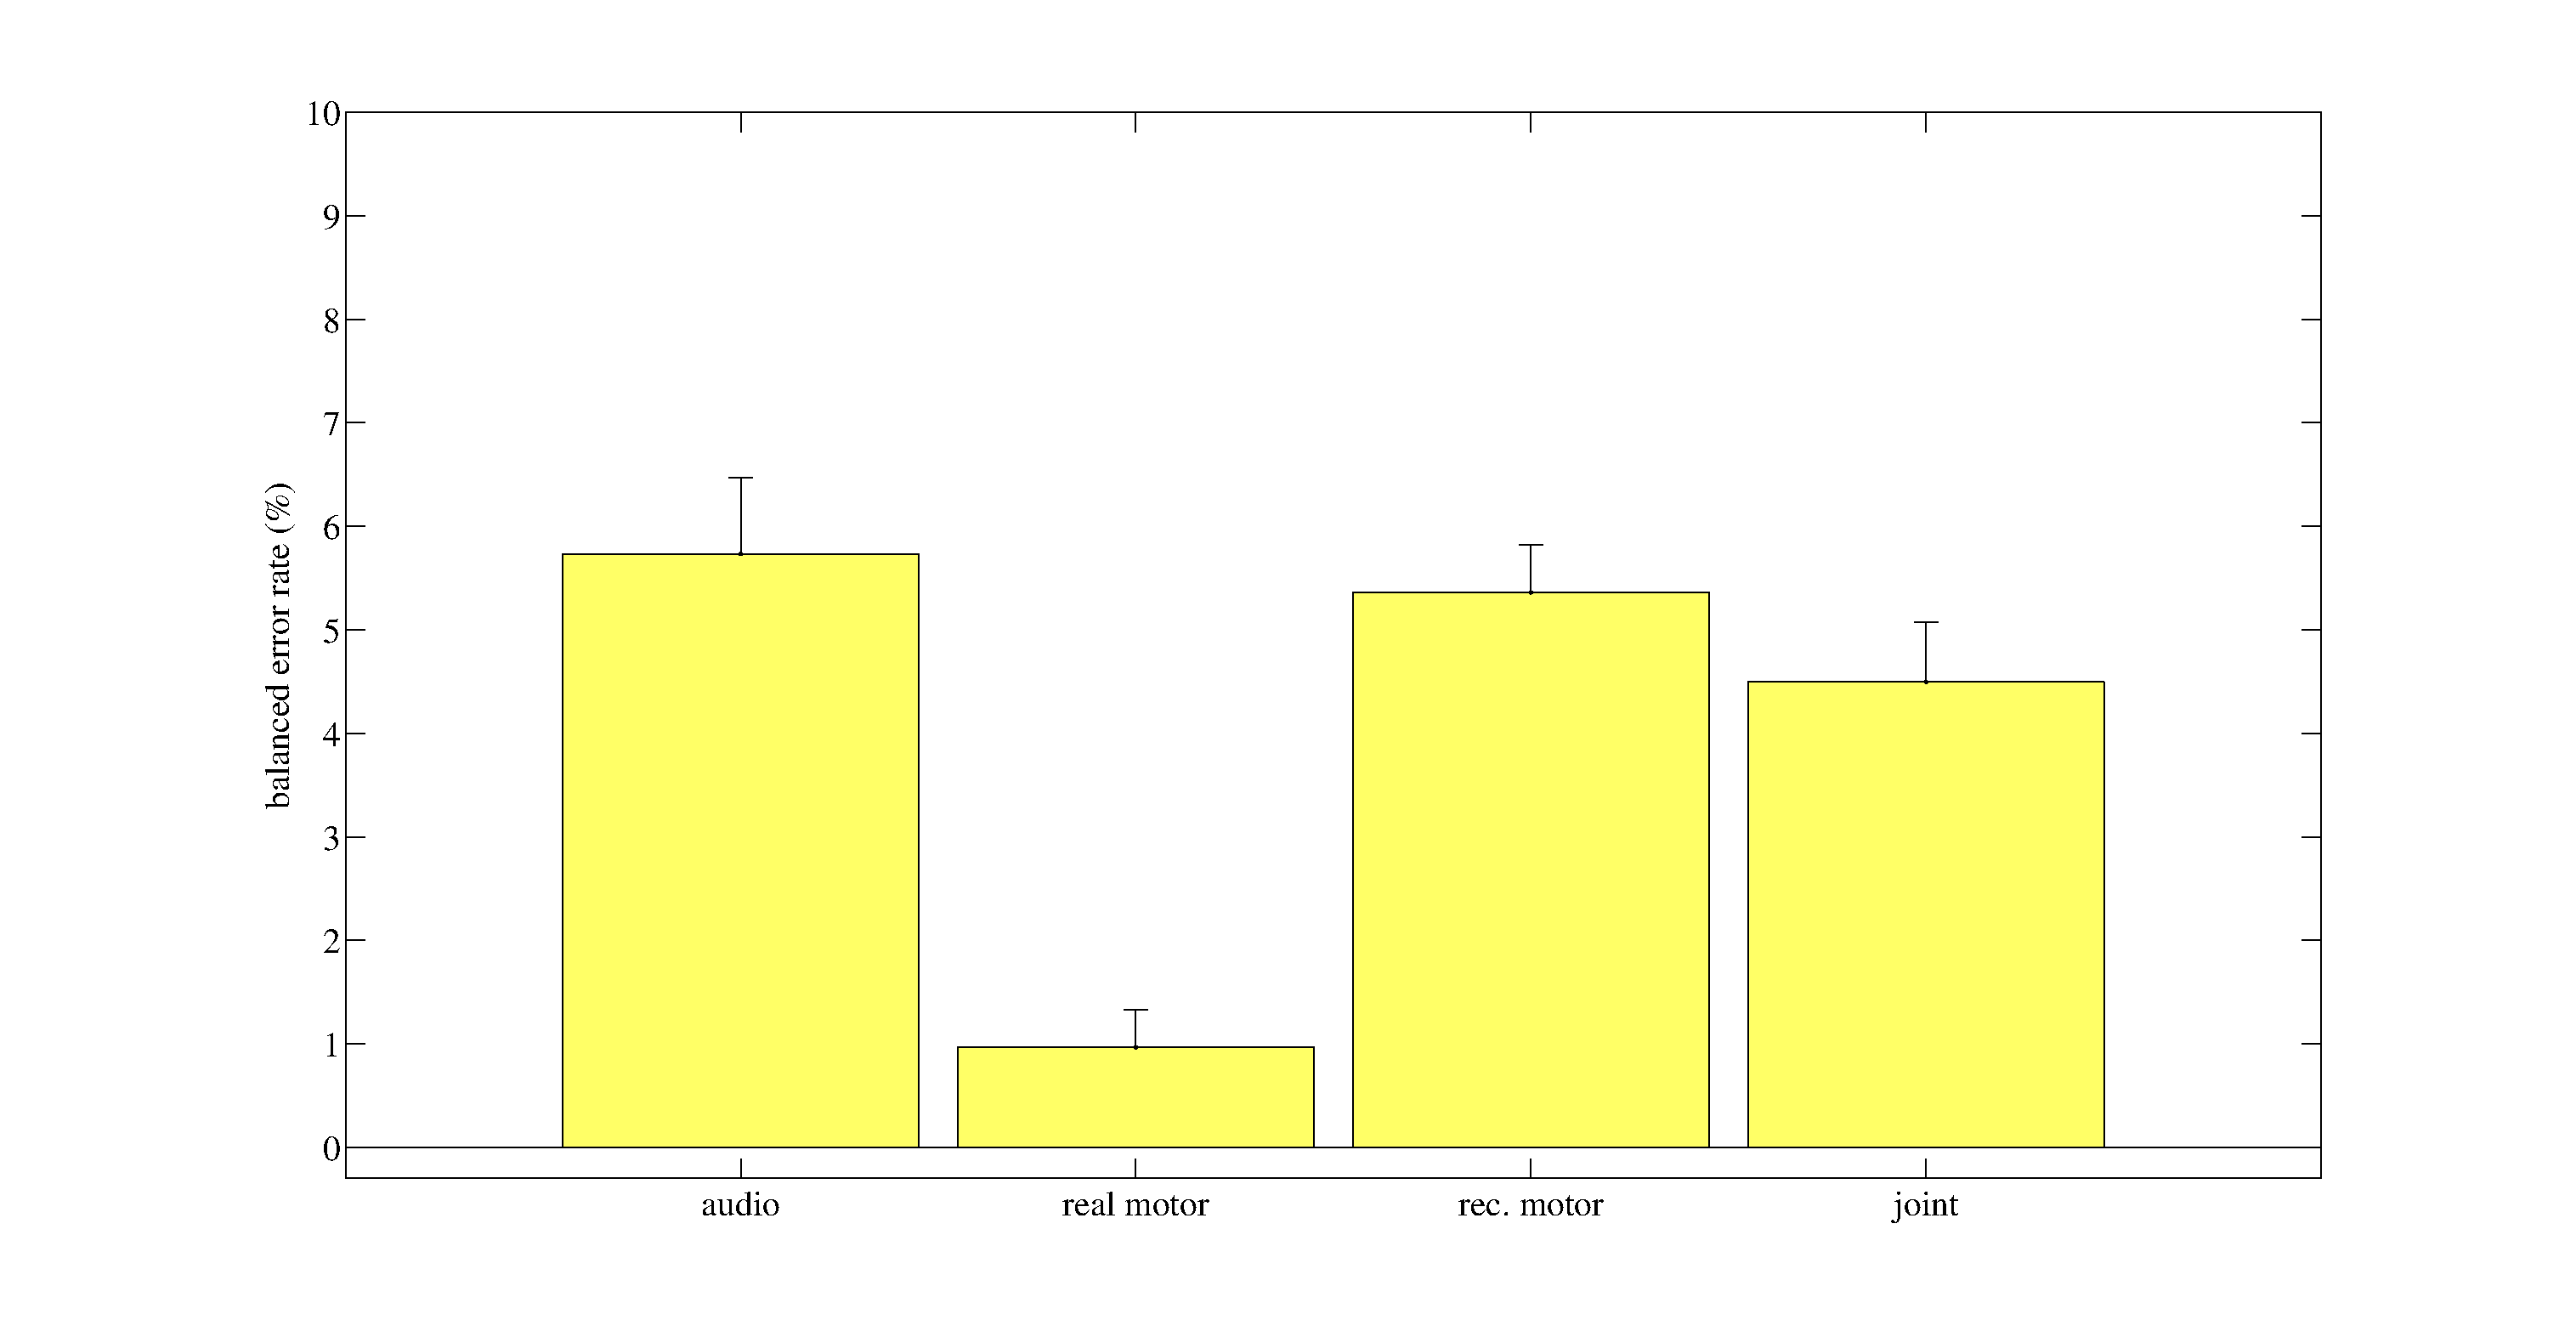
\includegraphics[width=0.95\linewidth]{figs/exp1}
  \caption{Classification results: Difference in performance between \emph{NoAdapt} and our method  on the
 classification of the grasp types.}
  \label{fig:diff_cla}
\end{figure}

\begin{figure*}[ht] \centering
  \begin{tabular}{cc}
    \includegraphics[width=0.45\textwidth]{figs/exp1_abs_best} &
    \includegraphics[width=0.45\textwidth]{figs/exp1_abs_worst} \\
    $(a)$ & $(b)$ \\
  \end{tabular}
  \caption{Classification results: $(a)$ Best classification rate gain of the adapted model compared to
 \emph{NoAdapt} and \emph{Prior} on a particular subject; $(b)$ worst performance on another subject.}
  \label{fig:cla_abs}
\end{figure*}

\begin{figure}[ht]
  \centering
  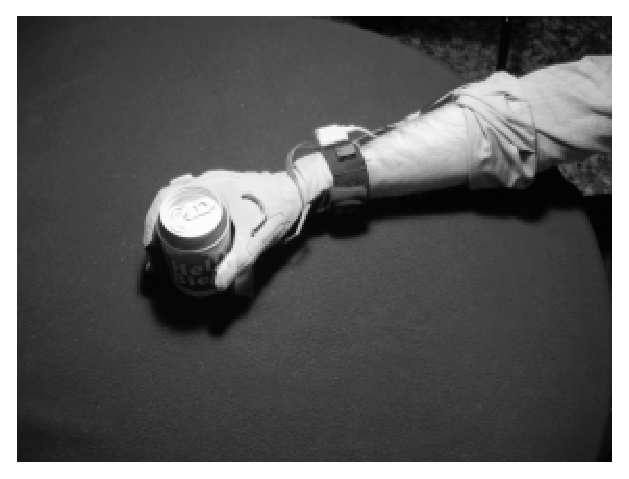
\includegraphics[width=0.95\linewidth]{figs/exp2}
  \caption{Regression experiments: Difference in performance between \emph{NoAdapt} and our method  on the
 regression of the force.}
  \label{fig:diff_reg}
\end{figure}

\begin{figure*}[ht] \centering
  \begin{tabular}{cc}
    \includegraphics[width=0.45\textwidth]{figs/exp2_abs_best} &
    \includegraphics[width=0.45\textwidth]{figs/exp2_abs_worst} \\
    $(a)$ & $(b)$ \\
  \end{tabular}
  \caption{Regression experiments: $(a)$ Best correlation coefficient gain of the adapted model compared to \emph{NoAdapt}
 and \emph{Prior} on a particular subject; $(b)$ worst performance on another subject.}
  \label{fig:reg_abs}
\end{figure*}


\section{Discussion and Conclusions}
\label{sec:discussion}
Our experimental results, performed on a large data set of about
$153,000$ samples, clearly show that Online Uniformisation can be used
to obtain dramatically smaller training sets with no
\emph{qualitative} loss of information; in other words, as more of the
input space is sampled, OU keeps the training set up-to-date and
small. OU sets will result in small (and therefore, fast) and accurate
models of the sought-for EMG-to-hand map. Remarkably, OU works fine
for both grasp classification and force regression, and with all three
different machine learning approaches tested. Moreover, it is
extremely simple, being nothing more than an online check of Euclidean
distance in the input space. This check is done so far by considering
the new sample's distance from all samples in the current training
set, and therefore could become unfeasibly heavy as the set grows; but
the same check can be clearly done in constant time using an
algorithmic optimisation, such a hash table.

Moreover, OU will produce models which perform \emph{uniformly} well,
enabling a patient to drive the prosthesis with a good accuracy in
\emph{all} situations that might arise, no matter how frequently they
appear during the training phase.

The choice of the minimum inter-sample distance $d$ is obviously
crucial and depends on the required accuracy in classification and/or
regression; but as we have seen, as $d$ is increased, the machine's
performance degrades only linearly, whereas the training sets become
polynomially smaller. Therefore, at the price of having a slightly
worse performance, dramatically smaller training sets can be used.

To sum up, in this paper we have presented a machine learning
approach to joint classification of grasping and regression on the
applied force, using forearm surface electromyography. The approach is
totally non-invasive, easy to set up and use and it can be applied
from scratch with no previous knowledge of the problem. The Online
Uniformisation procedure can be used to incrementally build a training
set which will result in small and accurate models of the problem.

Our experiments, carried out using a Support Vector Machine with
Gaussian kernel, a Neural Network with sigmoidal activation function
and Locally Weighted Projection Regression, indicate that the approach
achieves, using a training set of about $1800$ samples on a total of
$153,000$ (for $d=0.21$), an average accuracy of around $90\%$ in
classification of grasp types and a normalised root MSE of $7.89\%$ in
prediction of the force applied during the grasp. Of the tested
approaches, SVM is marginally better than the others, especially when
larger training sets are used. The OU procedure is able to find as
small a training set as $77.4$ samples on average (out of $153,000$),
which will still result in a SVM having a remarkable NRMSE of
$12.12\%$.

\subsection*{Future work}

We believe this is the first step toward the real application of
machine learning to an EMG-driven adaptive, dexterous AHP. Let us
consider the problems outlined in section
\ref{subsubsec:electrodes}: in this paper we have solved problems
$3$ and $4$. Now, since OU lets us obtain good accuracy with extremely
small training sets, it is not too far-fetched to say that the
solution of problem $2$ is at hand --- in principle, the changing arm
posture can be taken into account simply by sampling more of the input
space. As far as problem $1$ is concerned, inter-subject usability is
really of lesser interest, since one patient only is supposed to ever
wear a prosthesis; on the other hand, multi-subject analysis has to be
carried out eventually, since it must be possible to obtain good
results on \emph{any} subject the method is applied to. We see no
reason, however, why this should not be the case, at least as far as
able-bodied subjects are concerned.

The ultimate problem is of coruse that of training the system upon
amputees. First of all, the patient must still have a good deal of
muscular and nervous plasticity in her arm stump; then, a smart way of
collecting training data must be devised --- an amputee is obviously
not expected to train the machine with a hand. A simple idea is that
of gathering EMG data from the patient's stump and grasping/force data
from her healthy hand, while instructing her to imagine doing the same
actions with both hands. Secondly, the issue of sensorial feedback
will have to be addressed, in order to provide the patient with
reliable information about the force actually involved in the
grasp. This is likely to be crucial in order to realise a tighter and
tighter loop between the patient and the prosthesis.

As far as force regression is concerned, the results presented above
are, to the best of our knowledge, totally novel. Surprisingly,
regression from the forearm surface EMG signal to the force applied by
the hand had never been attempted before. Given the good performance
obtained by our models, we claim that the relationship between the EMG
signal and the force has been captured by the models, under variable
conditions of muscle fatigue (within one session) and electrode
displacement (within sessions belonging to different groups). In a
certain sense, this work is an evolution of the so-called
\emph{proportional} control of myoelectric prostheses already
available on the market; in proportional control, the ``claw'' of the
prosthesis is actuated with a force which is proportional to the
amplitude of the EMG signal. In this case, the applied force is
proportional as well, but the control is realised in a totally natural
way, and is \emph{adaptive} to the user, what has never been done
before.


\section*{Acknowledgment}

The authors would like to thank...

\bibliographystyle{IEEEtran}
\bibliography{paper,claudio}

%% \begin{IEEEbiography}{Michael Shell}
%% Biography text here.
%% \end{IEEEbiography}

%% \begin{IEEEbiographynophoto}{John Doe}
%% Biography text here.
%% \end{IEEEbiographynophoto}

\end{document}
